\documentclass[tikz,border=6pt]{standalone}
\usepackage[T1]{fontenc}
\usepackage[utf8]{inputenc}
\usepackage{pgfplots}
\pgfplotsset{compat=1.18}
\begin{document}
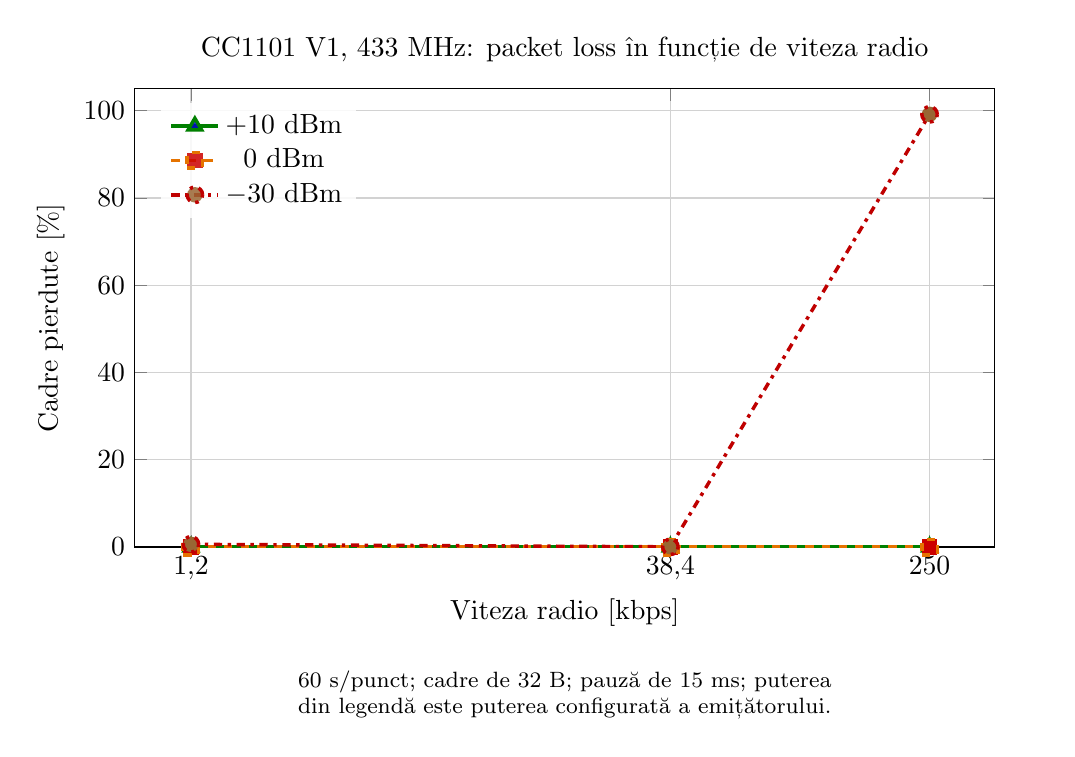
\begin{tikzpicture}
\begin{axis}[width=12.5cm, height=7.4cm,
  title={CC1101 V1, 433 MHz: packet loss în funcție de viteza radio},
  xmode=log, log basis x=10,
  xmin=0.8, xmax=400, xtick={1.2,38.4,250},
  xticklabels={1{,}2,38{,}4,250},
  ymin=0, ymax=105, ytick={0,20,40,60,80,100},
  xlabel={Viteza radio [kbps]}, ylabel={Cadre pierdute [\%]},
  grid=both, minor grid style={gray!15}, major grid style={gray!35},
  every axis plot/.append style={line width=1.25pt, mark size=2.8pt},
  legend style={draw=none, fill=white, fill opacity=0.85, text opacity=1,
    at={(0.03,0.97)}, anchor=north west, legend columns=1},
]
\addplot+[green!50!black, mark=triangle*] coordinates {(1.2,0.000000) (38.4,0.000000) (250,0.000000)};
\addlegendentry{+10 dBm}
\addplot+[orange!90!black, dashed, mark=square*] coordinates {(1.2,0.000000) (38.4,0.000000) (250,0.000000)};
\addlegendentry{0 dBm}
\addplot+[red!75!black, dashdotted, mark=*] coordinates {(1.2,0.617284) (38.4,0.046664) (250,99.160168)};
\addlegendentry{$-30$ dBm}
\end{axis}
\node[font=\footnotesize, align=center, text width=12cm, anchor=north]
  at ([yshift=-1.45cm]current axis.south)
  {60 s/punct; cadre de 32 B; pauză de 15 ms; puterea din legendă este puterea configurată a emițătorului.};
\end{tikzpicture}
\end{document}
